\section {Results}
\label{sec:results}

The classifiers developed in this replication attempt were constructed and evaluated according to the parameters
and metrics described in Section~\ref{sec:modelflex}. Figure~\ref{fig:7_class_model} shows the sensitivity
and specificity of each tested model alongside the performance of the originally published model, with 10\% of models
most closely matching performance to the reference highlighted.
Tables~\ref{tab:prob_7class} and~\ref{tab:prob_8class} contain the complete performance of the probability-based models
evaluated using each performance metric for the 7- and 8-class settings, respectively. Table~\ref{tab:scikit_pred}
shows the same for the SKlearn Prediction models.

Table~\ref{tab:dpcPhcAaindexPssm},~\ref{tab:aacDpcPhcAaindexPssm},~\ref{tab:dpcPhcAaindexPssmAaindexPhc},
~\ref{tab:aacDpcAaindexPssmHybrid3},~\ref{tab:aacAaindexPhcPssmHybrid3}
contain the evaluation of the best-performing models fit on AAC when 
applied across all the other 18 features. Figure~\ref{fig:MccAllModels} compared the MCC values resulted 
from running the the best-performing models on all the features. Finally, Table~\ref{tab:pssmAaindex} 
shows the results of running the best-performing models on the main and independent datasets for the 
hybrid model that included the biochemical composition and the PSSM profile.

\GK{For Hamid: regenerate data in the all-feature-performance table based on more than just the "best" model. At
present, we cannot include anything in the results about this because there isn't a result to discuss.}

The remainder of this section will explore the differences in model performance based on the defined axes of
flexibility enumerated in Section~\ref{sec:experimentaldesign}.

% Figure 1
\begin{figure}
  \centering
  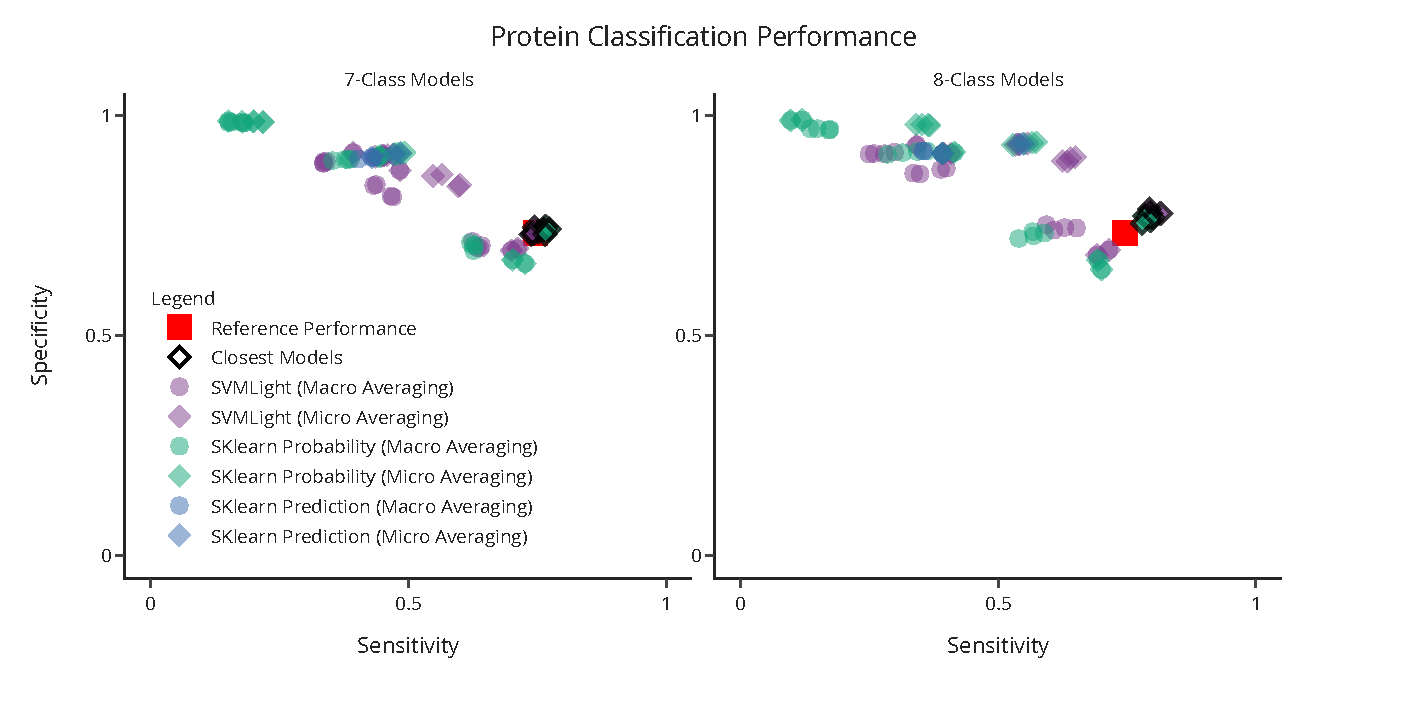
\includegraphics[width=\textwidth]{figures/fig1_model_performance.pdf}
  \caption{Sensitivity and Specificity of each tested model. Each panel contains models trained with a fixed number of
categories (7: left; 8: right), and shows the published reference performance in red. The closest 10\% of models to
this reference have been outlined in black. The symbol colour and shape refer to the classifier type and aggregation
strategy, respectively. Each shaded region illustrates the bounds of performance for a given binary classifier
aggregation strategy.}
   \label{fig:7_class_model}
\end{figure}

\paragraph{Number of Classes}
While the 7-class models appear to be slightly closer to the reference, there was no significant difference between
the number of classes and the distance from reference ($p > 0.1$). Models trained with 8 classes tended to achieve
higher sensitivity and specificity values, however, suggested improved performance with the addition of the background
class. 

\paragraph{Dataset Sampling}
The dataset composition had no significant impact on the closeness of the model to the reference ($p > 0.1$ for all
comparisons). However, none of the closest 10\% of models were trained using the downsampled dataset.

\paragraph{SVM Hyperparameters}
All uniformly parameterized models converged to same set of hyperparameters within the number of classes, where the
best performing 7-class models used Gamma and Cost values of $0.02$ and $4.5$ while 8-class models had best performance
with $0.01$ and $4$, respectively. There was no significant difference between these sets of parameters.

\paragraph{Hypterparamter Heterogeneity}
Similarly to the case of uniform parameters, models converged on Gamma values between $0.02$ and $0.04$ for all classes
and models, and Cost values between $4$ and $5$, with no statistically significant difference between models or classes.

\paragraph{Aggregation Technique}
Models using the micro performance-aggregation technique (i.e. evaluating individual binary classifiers prior to
aggregation into a multi-class classifier) obtained closer results to the reference than those using the macro
technique ($p < 1\times 10^{-4}$). All of the closest models used micro-aggregation.

\paragraph{Prediction Method}
The balanced averaging prediction method produced significantly closer results to the reference than both the
unweighted average and maximum probability methods ($p < 1\times 10^{-5}$ for both). The maximum probability method
also produced significantly closer results than the unweighted average method ($p < 0.001$).

\paragraph{Tool}
The SVMLight classifiers produced closer results to the reference than both SKlearn Probability and Prediction models
($p < 0.05$ for both). While the SKlearn Prediction model architecture did not appear in the set of closest models,
there was no statistically significant difference between its performance and that of the SKlearn Probability models.

\subsection{Closest Models}
The closest 10\% of models (16) used a variety of configurations, and each reported a distance score of less than
$0.13$ from the reference. The breakdown of configurations for these models included: micro aggregation (all), balanced
average prediction method (all), balanced (8) or shuffled (8) dataset, contained 7 (8) or 8 (8) classes in the dataset,
were trained with uniform (8) or heterogeneous (8) hyperparameters, and were developed using SVMLight (8) or the
SKlearn Probability (8) model architectures. While the SKlearn Prediction model and downsampled dataset configuration
are notably absent from these models, all other settings were either dominated by a single value, such as in the case
of micro aggregation and the balanced average prediction method, or the settings were equally represented. This
uniformity in representation is consistent with the direct comparisons between settings described above.

For all the other 18 feature sets (dpc, phc, pssm, aaindex and 14 hybrid feature sets) the closest 10\% of the models (16) 
each reported a distance score of less than $0.13$ from the feature's reference values. 
Figure~\ref{fig:MccAllModels} shows the MCC values resulted from running 
the closest 10\% models (16) on all the features (19). 
The hybrid dataset that included the biochemical composition (AAindex) and the PSSM profile 
outperforms others. For this feature set, the closest models (Table~\ref{tab:pssmAaindex}) reported 
the distance score of less than $0.09$ on the main dataset and less than $0.08$ on the independent dataset.

\GK{TODO Hamid: add results for the other analyses, such as 1- running the best 10\% of models on more features and
2- evaluating them on the independent dataset.}

% Table 1
